\documentclass[svgnames]{beamer}
%\documentclass[svgnames, handout]{beamer}

\usepackage{pnup}
\usepackage{pgfpages}

%\pgfpagesuselayout{3 on 1 with notes}[a4paper,border shrink=5mm]

\mode<handout>{\setbeamercolor{background canvas}{bg=black!5}}

\usefonttheme[onlymath]{serif}		% Display math in serif font

%\usepackage[svgnames]{xcolor}

\batchmode
% \usepackage{pgfpages}
% \pgfpagesuselayout{4 on 1}[letterpaper,landscape,border shrink=5mm]

\usepackage{amsmath,amssymb,color}

\usepackage{algorithmic}
\usepackage{algorithm}

\usepackage{multirow}	% Multiple rows and columns in tables
\usepackage{booktabs}	% Professional tables

% Math stuff
\newcommand{\xor}{\oplus}

\usetheme{Berlin}
\usecolortheme{bear}

\title{Compact implementations of pairings}
\author[Anthony Van Herrewege]{Anthony Van Herrewege\\[2em]
\footnotesize Day. sup.: Dr. Lejla Batina, Miroslav Knezevic, Dr. Ir. Nele Mentens\\
Prom.: Prof. Dr. Ir. Ingrid Verbauwhede, Prof. Dr. Ir. Bart Preneel\\
Ass.: Prof. Dr. Ir. Wim Dehaene, Dr. Ir. Frederik Vercauteren}
\date{22 May 2009}
%\pgfdeclareimage[height=1cm]{brown-logo}{brown-logo.pdf}
%\logo{\pgfuseimage{brown-logo}\hspace*{0.3cm}}

\newenvironment{changemargin}[2]{%
\begin{list}{}{%
\setlength{\topsep}{0pt}%
\setlength{\leftmargin}{#1}%
\setlength{\rightmargin}{#2}%
\setlength{\listparindent}{\parindent}%
\setlength{\itemindent}{\parindent}%
\setlength{\parsep}{\parskip}%
}%
\item[]}{\end{list}}

\AtBeginSection[]
{
  \begin{frame}<beamer>
    \frametitle{Outline}
    \tableofcontents[currentsection]
  \end{frame}
}
\beamerdefaultoverlayspecification{<+->}

\setbeameroption{show notes}

\begin{document}

\frame{\titlepage}

\section[Outline]{}
\begin{frame}{Outline}
  \tableofcontents
\end{frame}

\section{Pairings}
\subsection*{Pairings}
\begin{frame}{Overview}
	\begin{itemize}
		\item Several available pairings:
			\begin{center}Weil, \alert{Tate}, $\eta _T$, Ate, $\ldots$\end{center}
		
		\item	Bilinearity property:
			\[ e(P_1 + P_2, Q) = e(P_1, Q) \cdot e(P_2, Q) \]
	
		\item \emph{Optimized} Tate pairing:	
			\[\begin{gathered}
				\hat{e}(P, Q) : E(\mathbb{F}_q)[l] \times E(\mathbb{F}_q)[l] \mapsto \mu _l \\
				\mu _l = \text{group of $l$th roots of } \mathbb{F}_{q^k}^*
			\end{gathered}\]
	\end{itemize}
\end{frame}

\begin{frame}{Possibilities}
	\begin{itemize}
		\item Identity-based encryption
		\item Short signatures
		\item Non-interactive key agreement
		\item Tripartite key agreement in 1 round
		\item \ldots
	\end{itemize}
\end{frame}

\section{Implementation}
\subsection*{Implementation}
\begin{frame}{Restrictions}
Avoid the use of flip-flops and muxes:

	\begin{center}
	\begin{tabular}{lr}
		\toprule
		Cell							& Area $\left[\frac{\text{gate}}{\text{bit}}\right]$\\
		\midrule
		D flip-flop (reset)		& 6\\
		D flip-flop (no reset)	& 5.5\\
		D latch						& 4.25\\
		3 input MUX					& 4\\
		2 input XOR					& 3.75\\
		2 input MUX					& 2.25\\
		2 input NAND				& 1\\
		NOT							& 0.75\\
		\bottomrule
	\end{tabular}
	\end{center}
\end{frame}

\begin{frame}{MALU - Addition \& Reduction in $\mathbb{F}_{2^m}$}
\\[-1em]
	\[\begin{gathered}
		R = \left(T + B \quad (\text{mod } P_{\text{in}}) \right)_{0:m-2} \ll 1 \\
		mod_{\text{u}} = \left(T + B \quad (\text{mod } P_{\text{in}}) \right)_{m - 1}
	\end{gathered}\]
	\begin{changemargin}{-2cm}{-2cm}
	\begin{center}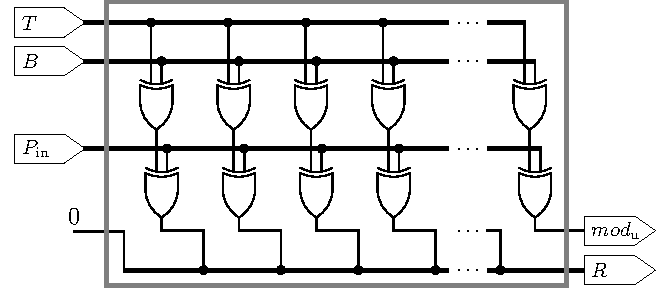
\includegraphics[height=0.5\paperheight]{images/malu-basic}\end{center}
	\end{changemargin}
\end{frame}

\begin{frame}{MALU - Addition \& Reduction in $\mathbb{F}_{2^m}$}
	Optimized MALU needs $\Delta = m - \left( \textsf{Hamm}(P) - 1 \right)$ less XORs:\\[1.7em]
	\begin{changemargin}{-2cm}{-2cm}
	\begin{center}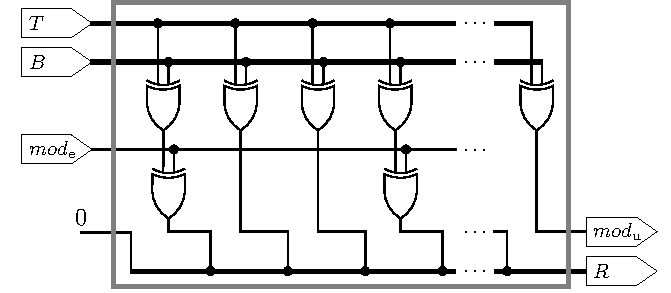
\includegraphics[height=0.5\paperheight]{images/malu-optimized}\end{center}
	\end{changemargin}
\end{frame}

\begin{frame}{$\mathbb{F}_{2^m}$ Multiplication \& Addition}
	\begin{changemargin}{-4cm}{-4cm}
		\begin{center}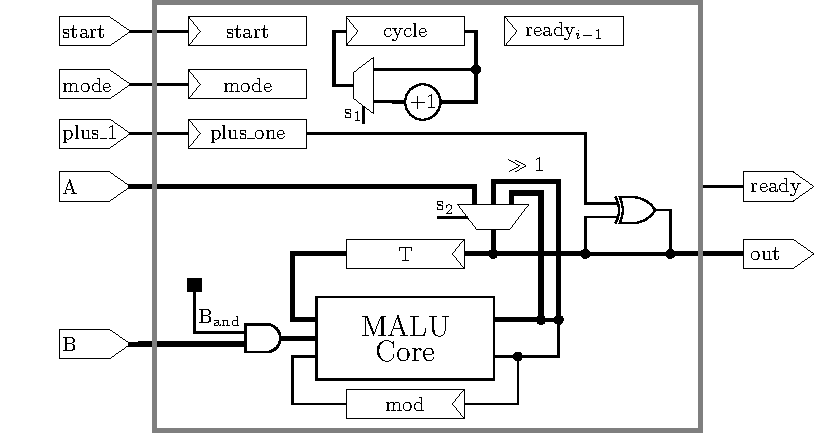
\includegraphics[height=0.65\paperheight]{images/wrapper-gf2m}\end{center}
	\end{changemargin}
\end{frame}

\begin{frame}{$\mathbb{F}_{2^m}$ Multiplication \& Addition}
	No FSM needed, simple logic:\\[0.7em]
	\begin{changemargin}{-4cm}{-4cm}
		\begin{center}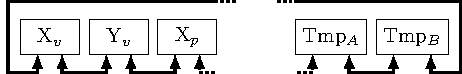
\includegraphics[height=0.55\paperheight]{images/wrapper-gf2m-logica}\end{center}
	\end{changemargin}
\end{frame}

\begin{frame}{$\mathbb{F}_{2^m}$ Multiplication \& Addition}
	Speed up calculation by daisy-chaining MALUs ($m \bmod d$!):\\[0.7em]
	\begin{changemargin}{-1cm}{-1cm}
	\begin{center}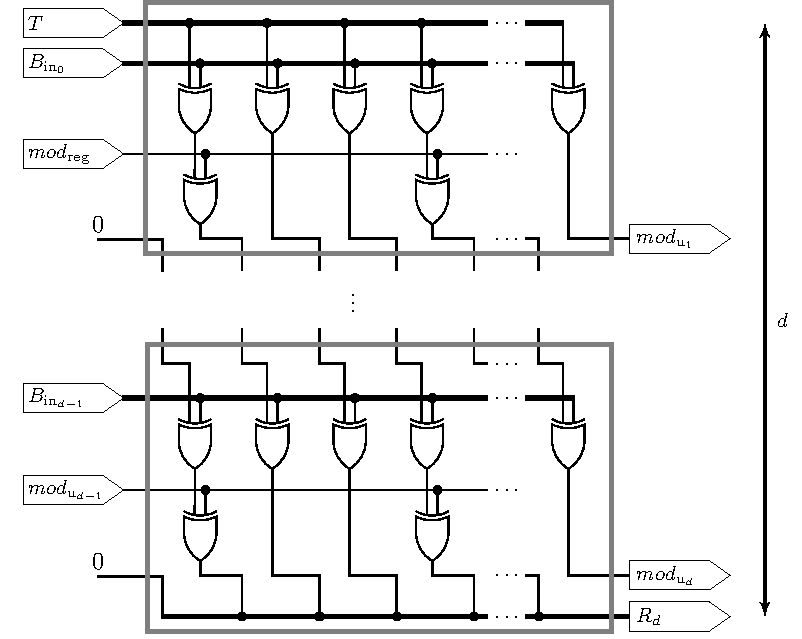
\includegraphics[height=0.6\paperheight]{images/malu-width-d}\end{center}
	\end{changemargin}
\end{frame}

\begin{frame}{Controller for Miller's algorithm}
\vfill
	\begin{changemargin}{-4cm}{-4cm}
		\begin{center}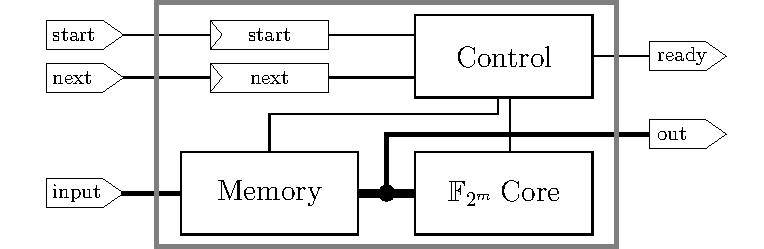
\includegraphics[width=1\paperwidth]{images/controller-miller}\end{center}
	\end{changemargin}
\vfill
\end{frame}

\begin{frame}{Memory design}
	Initial design:
	\[\overline{t} = O \left( \frac{n^2}{3} \right) \quad \qquad \overline{w} = O \left( \frac{n^3}{3} \right)\] \\[1.7em]
	
	\begin{changemargin}{-4cm}{-4cm}
		\begin{center}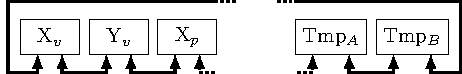
\includegraphics[width=0.8\paperwidth]{images/geheugen-circ}\end{center}
	\end{changemargin}
\end{frame}

\begin{frame}{Memory design}
	Final design:\\[0.3em]
	\[\overline{t} = O \left( \frac{n}{4} \right) \quad \qquad \overline{w} = O \left( n \right)\] \\[1.7em]
	
	\begin{changemargin}{-4cm}{-4cm}
		\begin{center}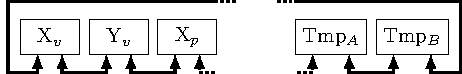
\includegraphics[width=0.8\paperwidth]{images/geheugen-circ-optimized}\end{center}
	\end{changemargin}
\end{frame}

\begin{frame}{Optimizations}
	\begin{itemize}
		\item Remove reset from registers $\left( -0.5 \: \frac{\text{gate}}{\text{bit}} \right)$
		\item Implement clock gating:
	\end{itemize}
	
	\begin{changemargin}{-2cm}{1.2cm}
		\raggedleft
			\uncover<3->{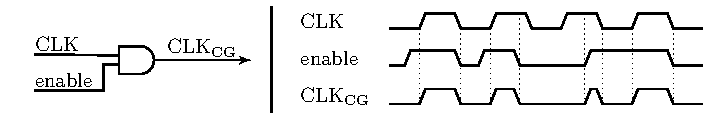
\includegraphics[height=0.13\paperheight]{images/cg-basic}} \\[0.7em]
			\uncover<4->{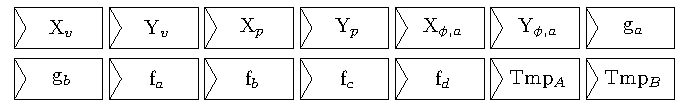
\includegraphics[height=0.1747\paperheight]{images/cg-no-glitch}} \\[0.7em]
			\uncover<5->{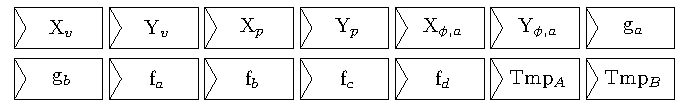
\includegraphics[height=0.13\paperheight]{images/cg-low-power}}\\
	\end{changemargin}
\end{frame}

\section{Results}
\subsection*{Results}
\begin{frame}{Runtime}
	\begin{itemize}
		\item FSM with 553 states
		\item Total n$^{\circ}$ of clock cycles $c$ for one pairing:
				\[c = 21681 + 4322 + 2998 \cdot \left\lceil \frac{m}{d} \right\rceil\]
	\end{itemize}
	
	\begin{changemargin}{-4cm}{-4cm}
		\begin{center}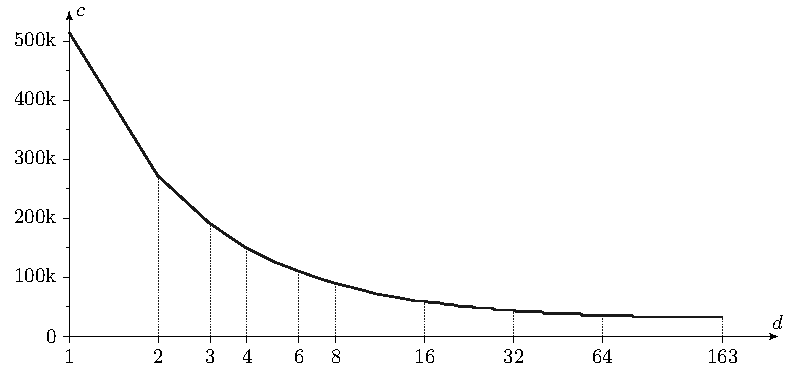
\includegraphics[height=0.40\paperheight]{images/results-multi-cycles}\end{center}
	\end{changemargin}
	
	~\\[3em]
	
\vfill
\end{frame}

\begin{frame}{Synthesis}
	\begin{center}
		\tiny{\begin{tabular}{llrlrlr}
			\\[-2em]
			\toprule
			\multirow{2}{*}{Implementation}	& \multicolumn{2}{c}{\multirow{2}{*}{Area [gates]}}	& \multicolumn{4}{c}{Power @ 10 kHz [$nW$]}\\
			\cmidrule{4-7}
			&	& & \multicolumn{2}{c}{Dynamic}	& \multicolumn{2}{c}{Leakage}\\
			\midrule
			Basic			& $28\,876$	& 			& $512$	&	 		& $117$ 	& \\
			No Reset		& $27\,596$	& $96\%$	& $395$	& $77\%$	& $107$ 	& $92\%$\\
			CG 1			& $27\,751$	& $96\%$	& $94$	& $18\%$	& $109$	& $94\%$\\
			CG 2			& $27\,713$	& $96\%$	& $59$	& $12\%$	& $102$	& $88\%$\\
			CG 3			& $27\,734$	& $96\%$	& $96$	& $19\%$	& $110$	& $94\%$\\
			\bottomrule		
		\end{tabular}}

		\\[2em]

		\begin{changemargin}{-1cm}{-1cm}\begin{center}
			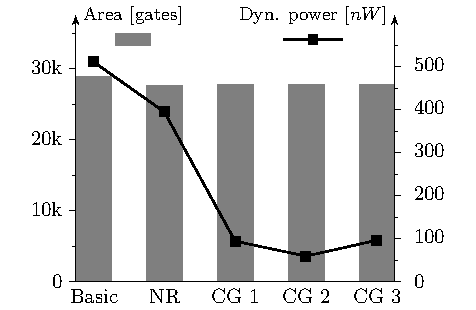
\includegraphics[width=0.45\paperwidth]{images/results-m1-en}
		\end{center}\end{changemargin}
	\end{center}
\end{frame}

\begin{frame}{Synthesis - Continued}
\vfill
	\begin{center}
	\begin{changemargin}{-0.3cm}{-0.8cm}
		\begin{minipage}[c]{0.3\paperwidth}
			\tiny{\begin{tabular}{llr}
				\toprule
				Component					& \multicolumn{2}{c}{Opp. [gates]}\\
				\midrule
				MALU				 			& $458$		& $1.7\%$\\
				$\mathbb{F}_{2^m}$ core	&				& \\
				$\quad$ Logic				& $783$		& $2.8\%$\\
				$\quad$ Registers			& $962$		& $3.5\%$\\
				Controller					&				& \\
				$\quad$ Logic				& $13\,044$	& $47\%$\\
				$\quad$ Registers			& $12\,487$	& $45\%$\\
				\midrule
				Total						& $27\,734$	& $100\%$\\
				\bottomrule		
			\end{tabular}}
		\end{minipage}
		\hfill
		\begin{minipage}{0.60\paperwidth}
			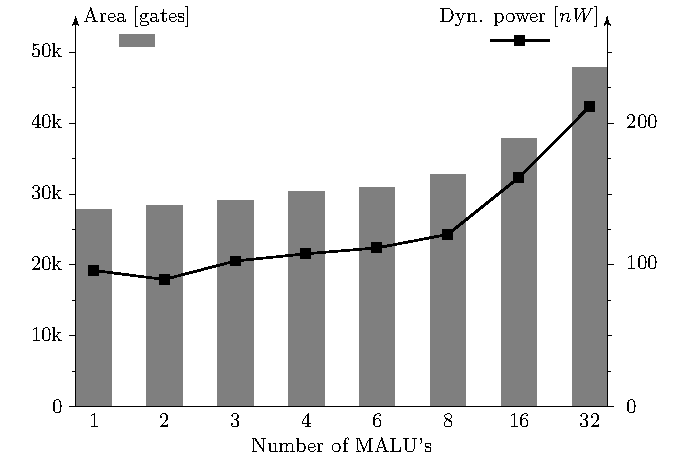
\includegraphics[width=0.60\paperwidth]{images/results-md-en}
		\end{minipage}		
	\end{changemargin}
	\end{center}
\vfill
\end{frame}

\begin{frame}{Comparison}
\begin{center}
\small{\begin{tabular}{llll}
			\\[-1.5em] \toprule
			&	\multicolumn{2}{c}{This work}	& \multirow{2}{*}{$\begin{array}{@{}c@{}}\text{Beuchat}\\\text{\emph{et al.}}\end{array}$}\\
			\cmidrule(r){2-3}
			& \multicolumn{1}{c}{1 MALU} & \multicolumn{1}{c}{2 MALUs} &\\
	 		\midrule
			Field																& $\mathbb{F}_{2^{163}}$	& $\mathbb{F}_{2^{163}}$	& $\mathbb{F}_{3^{97}}$\\
			Pairing															& Tate							& Tate							& $\eta_T$\\
			Security $[$bit$]$											& $652$							& $652$							& $922$\\
			Technology $[\mu m]$											& $0.13$							& $0.13$							& $0.18$\\
			Area $[$gates$]$												& $27\,430$						& $28\,155$						& $193\,765$\\
			$f$ $[$MHz$]$													& $10.3$							& $5.44$							& $200$\\
			Calc. time $[\mu s]$											& $50 \cdot 10^3$				& $50 \cdot 10^3$				& $46.7$\\
			Power $[mW]$													& $98.3 \cdot 10^{-3}$		& $48.6 \cdot 10^{-3}$		& $672$\\
			Efficiency $\left[ \frac{nJ}{\text{bit}}\right]$	& $7.54$							& $3.73$							& $34.0$\\
			\bottomrule		
		\end{tabular}}
		
		\\[1.5em]
		
		Efficiency = $\frac{\text{power} \; \times \; \text{calc. time}}{\text{bits security}}$
\end{center}
\end{frame}

\begin{frame}{Conclusion}
	\begin{itemize}
		\item Very small: $< 30$k gates
		\item Extremely low power: $<220$ nA
		\item Energy efficiency improvement up to more than $25 \times$ possible
	\end{itemize}
	
	\\[1em]
	
	\begin{center}
		\uncover<4->{Definitely possible to use in constrained environments}
	\end{center}
	
	\begin{itemize}
		\item<5-> Example with 3 MALUs:
				\[\begin{aligned}
					&\text{Area} = 29\text{k gates} & \qquad &f = 9.70 \text{ Mhz}\\
					&\text{Power = } 100 \text{ } \mu \text{A} \quad & \qquad &\text{Time = } 19.6 \text{ ms}
				\end{aligned}\]
	\end{itemize}
\end{frame}

\begin{frame}{The end}
	\begin{center}\LARGE Questions?\end{center}
\end{frame}

\end{document}
